\documentclass{beamer}

% \usepackage[utf8]{inputenc}
% \usepackage[T1]{fontenc}
\usepackage{lmodern}   % modern Latin Modern fonts
\usepackage{textcomp}  % provides \textquoteright
\usepackage{lmodern} % Latin Modern fonts with T1 shapes


\usepackage{graphicx}
\usepackage{ragged2e} % for generating dummy text
\usepackage[backend=biber,style=authoryear]{biblatex}
% \addbibresource{references.bib}

\usetheme{Madrid}
\usecolortheme{default}
\usefonttheme{professionalfonts} % keeps proper math fonts

\usepackage{amsmath,amssymb,amsfonts} % math symbols (\mathcal, \mathbb, etc.)
\usepackage{mathrsfs}                 % optional: \mathscr for fancy script

% \setbeamercovered{invisible} 
\setbeamercovered{transparent}


\title{MF921 Topics in Dynamic Asset Pricing}
\subtitle{Week 3}
\author{Yuanhui Zhao}
\date{Boston University}

\begin{document}
\frame{\titlepage}
% \begin{frame}
% \frametitle{Outline}
% \tableofcontents
% \end{frame}
\section{Part I}
\begin{frame}{Part I}
    \begin{center}
        Option Pricing Under a Double Exponential Jump Diffusion Model
    \end{center}
    \vspace{2em}
    \begin{center}
        S.G. Kou\\
        Hui Wang
    \end{center}
    \vspace{3em}
    \par This paper aims to show that a double exponential jump diffusion model can lead to an analytic approximation for finite-horizon
    American options and analytical solutions for popular path-dependent options (such as lookback, barrier, and perpetual American options). We will focus on lookback and barrier options here.
 \end{frame}

 \section{Part II}
\begin{frame}{Part II}

    \begin{center}
        Pricing Path-Dependent Options with Jump Risk via Laplace Transforms
    \end{center}
    \vspace{2em}
    \begin{center}
        Steven Kou\\
        Giovanni Petrella\\
        Hui Wang
    \end{center}
    \vspace{3em}
    \par  Show the analytical solutions for two-dimensional Laplace transforms of barrier option prices,
     as well as an approximation based on Laplace transforms for the prices of finite-time horizon American options, under a double exponential jump diffusion model.
    
\end{frame}


\section{Background}
\begin{frame}{Background}

    {\footnotesize \footnotesize
    \par Recall The Double Exponential Jump Diffusion Model:
    \begin{align*}
        \frac{dS(t)}{S(t^{-})} = \mu dt + \sigma dW(t) + d\left(\sum_{i=1}^{N(t)} (V_i - 1)\right)
    \end{align*}
    \par\begin{itemize}
    \item \( W(t) \): Brownian motion under the real-world measure.
    \item \( N(t) \): Poisson process with rate \(\lambda\).
    \item \( V_i \): multiplicative jump sizes, i.i.d. random variables.
    \item \( Y = \log(V) \), the jump sizes follow double exponential law:
    \end{itemize}   
    \begin{align*}
        f_Y(y) = p \eta_1 e^{-\eta_1 y} \mathbf{1}_{y \geq 0} + q \eta_2 e^{\eta_2 y} \mathbf{1}_{y < 0}
    \end{align*}
    \par with parameters:
    \begin{itemize}
        \item \( p, q \geq 0, p + q = 1 \): probabilities of upward/downward jumps.
        \item \(\eta_1 > 1\): rate for upward jumps.
        \item \(\eta_2 > 0\): rate for downward jumps.
    \end{itemize}
    }
    
\end{frame}

\begin{frame}{Background Con.}

    {\footnotesize \footnotesize
    \par For option pricing, we switch to a risk-neutral measure \( P^* \), so that the discounted price process is a martingale:
    \begin{align*}
        E^{P^*}[e^{-rt}S(t)] = S(0)
    \end{align*}
    \par Under \( P^* \), the dynamics adjust:
    \begin{align*}
        \frac{dS(t)}{S(t^-)} = (r - \lambda^*(t)\zeta^*)dt + \sigma dW^*(t) + d\left(\sum_{i=1}^{N^*(t)}(V_i^*-1)\right)
    \end{align*}
    \par where:
    \begin{itemize}
        \item \( W^*(t) \): Brownian motion under \( P^* \),
        \item \( N^*(t) \): Poisson process with intensity \( \lambda^* \),
        \item \( V^* = e^{Y^*} \): jump multiplier with new parameters \( (p^*, q^*, \eta_1^*, \eta_2^*) \),
        \item \( \zeta^* = E^{P^*}[V^*] - 1 = \frac{p^{*}\eta_{1}^{*}}{\eta_{1}^{*}-1} + \frac{q^{*}\eta_{2}^{*}}{\eta_{2}^{*}+1} - 1\) is mean percentage jump size.
    \end{itemize}
    \par The log-price process:  
    \begin{align*}
        X(t) = \log\left(\frac{S(t)}{S(0)}\right) = \left(r - \frac{1}{2}\sigma^2 - 
    \lambda^*\zeta^*\right)t + \sigma W^*(t) + \sum_{i=1}^{N^*(t)} Y_i^*,\;\;X(0)=0
    \end{align*}
    }
    
    
\end{frame}


\section{Intuition}
\begin{frame}{Intuition of the Pricing Formula}

    \begin{itemize}
    \item Without jumps, the model reduces to geometric Brownian motion. Pricing American, 
    barrier, and lookback options is straightforward. First passage times are tractable, and 
    closed-form formulas are well known (as what we show in last week).
    \vspace{1em}
    \item With jumps, however, analytical pricing becomes difficult 
    because the process can cross barriers by jumping over them (Overshoot Problem).
\end{itemize}
    
\end{frame}

\section{Intuition}
\begin{frame}{Intuition of the Pricing Formula Con}


     {\footnotesize \footnotesize
    \par Define the first passage time:
    \begin{align*}
        \tau_{b} := \inf\{t \geq 0 : X(t) \geq b\}, \quad b > 0
    \end{align*}
    \par In a jump diffusion, when the process crosses \( b \), it may overshoot: $X(\tau_{b}) - b > 0$.
    \vspace{1em}
    \par This overshoot creates complications to compute the distribution of the first passage
times analytically: 
    \begin{itemize}
        \item Need the distribution of overshoot \( X(\tau_{b}) - b \).
        \item Need the joint dependence between overshoot and \( \tau_{b} \).
        \item Need correlation between overshoot and the terminal state \( X(T) \)
    \end{itemize}
    \vspace{1em}
    \par \textbf{Note}: Double exponential distribution assumption has a memoryless property, this property 
    simplifies the overshoot distribution and allows tractable Laplace transforms of first passage times.
    }
    
\end{frame}

\section{Some Useful Formulas}
\begin{frame}{Some Useful Formulas}

    {\footnotesize \footnotesize
    \par The double exponential jump diffusion process is a special 
    case of L\'evy processes with two-sided jumps, whose characteristic exponent admits the (unique) representation: 
    \vspace{1em}
    \begin{align*}
    \phi(\theta) = E[e^{i\theta X_1}] = \exp\left\{i\gamma\theta - \frac{1}{2}A\theta^2 
    + \int_{-\infty}^{\infty}(e^{i\theta y} - 1 - i\theta y I_{\{|y|\leq 1\}})\Pi(dy)\right\}
    \end{align*}\vspace{1em}
    \par where the generating triplet $(\gamma, A, \Pi)$ is given by:
    \vspace{1em}
    \begin{itemize}
        \item $A = \sigma^2$
        \item $\Pi(dy) = \lambda \cdot f_Y(y)dy 
        = \lambda p \eta_1 e^{-\eta_1 y} I_{\{y\geq 0\}} dy + \lambda q \eta_2 e^{\eta_2 y} I_{\{y<0\}} dy$
        \item $\gamma = \mu + \lambda E[V I_{\{|V|\leq 1\}}] = \mu + \lambda p \left( \frac{1 - e^{-\eta_1}}{\eta_1} 
        - e^{-\eta_1} \right) - \lambda q \left( \frac{1 - e^{-\eta_2}}{\eta_2} - e^{-\eta_2} \right)$
    \end{itemize}
    
    
    }

    
\end{frame}

\begin{frame}{Some Useful Formulas Con}

    {\footnotesize \footnotesize
    \par Moment Generating Function of the log-price process, \( X(t) \):
    \begin{align*}
        \mathbb{E}^* \left[ e^{\theta X(t)} \right] = \exp\{G(\theta)t\}
    \end{align*}
    \par Where the function $G(\cdot)$ is defined as:
    \begin{align*}
        G(x) = x \left( r - \frac{1}{2} \sigma^2 - \lambda \zeta \right) + \frac{1}{2} x^2 \sigma^2 
        + \lambda \left( \frac{p \eta_1}{\eta_1 - x} + \frac{q \eta_2}{\eta_2 + x} - 1 \right)
    \end{align*}
    \par \textbf{Note}: Lemma 3.1 in Kou and Wang (2003) shows that the 
    equation \( G(x) = \alpha, \forall \alpha > 0 \), has exactly 
    four roots: \(\beta_{1,\alpha}\), \(\beta_{2,\alpha}\), \(-\beta_{3,\alpha}\), and \(-\beta_{4,\alpha}\), where: 
    \begin{align*}
        0 &< \beta_{1,\alpha} < \eta_1 < \beta_{2,\alpha} < \infty\\
        0 &< \beta_{3,\alpha} < \eta_2 < \beta_{4,\alpha} < \infty
    \end{align*}
    \par These roots determine the structure of Laplace transforms for first passage times.
    }
    
\end{frame}
\begin{frame}{Some Useful Formulas Con}

    {\footnotesize \footnotesize
    \par Infinitesimal Generator of the log-price process, \( X(t) \):
    \vspace{1em}
    \begin{align*}
        (\mathcal{L}V)(x) = \frac{1}{2}\sigma^2 V''(x) + \left(r - \frac{1}{2}\sigma^2 
        - \lambda\zeta\right)V'(x) + \lambda \int_{-\infty}^{\infty}\left(V(x+y) - V(x)\right)f_Y(y)\,dy
    \end{align*}
    \vspace{1em}
    \par The generator describes how expectations of functions of \( X(t) \) evolve in time:
    \vspace{1em}
    \begin{align*}
        \frac{d}{dt}\mathbb{E}[V(X_t)] = \mathbb{E}[(\mathcal{L}V)(X_t)]
    \end{align*}
    \vspace{1em}
    \par They provide the mathematical foundation to derive option pricing formulas.



    }
    
\end{frame}

\section{Pricing Path-Dependent Options}
\begin{frame}{Lookback Options}

    {\footnotesize \footnotesize
    \par Consider a lookback put option with an initial "prefixed maximum" \( M \geq S(0) \):
    \vspace{1em}
    \begin{align*}
        LP(T) &= \mathbb{E}^{\mathbb{P}^*} \left[ e^{-rT} \left( \max\{M, \max_{0 \leq t \leq T} S(t)\} - S(T) \right) \right]\\
        & =   \mathbb{E}^{\mathbb{P}^*}\left[ e^{-rT} \max\{M, \max_{0 \leq t \leq T} S(t)\} \right] - S(0)\\
    \end{align*}

    \par You need the joint distribution of $\max S(t)$ and $S(T)$, which is complicated for jump processes. 
    Laplace transforms convert a complicated path integral over time into a function of roots of $G(x)$
    which we can solve algebraically.
    }
    
\end{frame}

\begin{frame}{Lookback Options Con.}

    \par Theorem:
    {\footnotesize \footnotesize
    
    \vspace{1em}
    \par Using the notations \(\beta_{1,\alpha+r}\) 
    and \(\beta_{2,\alpha+r}\) as in early silde, the Laplace transform of the lookback put is given by:
    \vspace{1em}
    {\footnotesize \tiny
    \begin{align*}
        \hat{L}(T) = \int_0^\infty e^{-\alpha T} \mathrm{LP}(T)  dT = \frac{S(0)A_\alpha}{C_\alpha} \left( \frac{S(0)}{M} \right)^{\beta_{1,\alpha+r}-1} 
        + \frac{S(0)B_\alpha}{C_\alpha} \left( \frac{S(0)}{M} \right)^{\beta_{2,\alpha+r}-1}  
        + \frac{M}{\alpha+r} - \frac{S(0)}{\alpha}
    \end{align*}
    }
    \vspace{1em}
    \par For all \(\alpha > 0\); here:
    \vspace{1em}
    \begin{align*}
        A_\alpha &= \frac{(\eta_1 - \beta_{1,\alpha+r}) \beta_{2,\alpha+r}}{\beta_{1,\alpha+r} - 1} \\
        B_\alpha &= \frac{(\beta_{2,\alpha+r} - \eta_1) \beta_{1,\alpha+r}}{\beta_{2,\alpha+r} - 1}\\
        C_\alpha &= (\alpha + r) \eta_1 (\beta_{2,\alpha+r} - \beta_{1,\alpha+r})
    \end{align*}

    }
    
\end{frame}

\begin{frame}{Lookback Options Con.}


    {\footnotesize \footnotesize
    \par Laplace inversion: 
    \begin{align*}
        LP(T)  = \frac{1}{2\pi i} 
        \int_{c-i\infty}^{c+i\infty} e^{\alpha T} \hat{L}(\alpha)  d\alpha
    \end{align*}
    \par This is the Bromwich inversion integral, intractable in closed form.
     So we approximate it numerically. 
     \par The most widely used numerical methods for Laplace transform inversion is
     Gaver-Stehfest (GS) algorithm. Suppose you know the Laplace transform of a function \( f(t) \):
     \begin{align*}
        F(\alpha) = \int_{0}^{\infty} e^{-\alpha t} f(t)  dt
     \end{align*}
     \par The GS method approximates \( f(t) \) by evaluating \( F(\alpha) \) at carefully 
     chosen points along the real line.

    }
    
\end{frame}

\begin{frame}{Lookback Options Con.}


    {\footnotesize \footnotesize
    \par The formula is:
    \begin{align*}
        f(t) \approx \frac{\ln(2)}{t} \sum_{k=1}^{n} w_k F \left( \frac{k \ln(2)}{t} \right)
    \end{align*}

where:

\begin{itemize}
    \item \( n \) is an even integer (typically converges nicely even for n between 5 and 10).
    \item \( w_k \) are weights (depending only on \( n \) and \( k \)):
    \begin{align*}
        w_k = (-1)^{\frac{n}{2}+k} \sum_{j=\lceil k/2 \rceil}^{\min(k,n/2)} 
        \frac{j^{n/2}(2j)!}{(\frac{n}{2}-j)! j! (j-1)! (k-j)! (2j-k)!}
    \end{align*}
\end{itemize}
\par Intuition: The algorithm generates a sequence \( f_n(x) \) such that \( f_n(x) \to f(x),  n \to \infty \)

    }
\end{frame}


\begin{frame}{Lookback Options Con.}


    {\footnotesize \footnotesize
    \par Another method:
    \vspace{1em}
    \par We shall invert the transform in the complex domain by using the Euler inversion algorithm
     (EUL) developed by Abate and Whitt (1995), rather than in the real domain by the Gaver--Stehfest algorithm (GS). 
    \vspace{1em}
    \par The main reason for this is that the EUL inversion (which is carried out in the complex-domain) does not require the high numerical precision of the GS: A precision of 12 digits will suffice for the EUL, compared with the 80 
    digits accuracy required by the GS. The EUL algorithm is made possible partly due to an explicit formula 
    for the roots of \( G(x) \).
    \vspace{1em}
    \par The statistical results show that the difference between the EUL and GS results are small. So the  the EUL implementation is preferable, 
    since it's simple to implement, and it converges fast without requiring high numerical precision as in the GS.
    }   
    
    
\end{frame}

\begin{frame}{Barrier Options}


    {\footnotesize \footnotesize
    \par Consider the up-and-in call (UIC) option with the barrier level $H$ ($H>S(0)$):
    \vspace{1em}
    \begin{align*}
        UIC = E^{\mathbb{P}^*}[e^{-rT}(S(T) - K)^+I{\{ \max\limits_{0 \leq t \leq T} S(t) \geq H \}}]
    \end{align*}
    \vspace{1em}
    \par For any given probability \( P \), define:
    \vspace{1em}
    \begin{align*}
        \Psi(\mu, \sigma, \lambda, p, \eta_1, \eta_2; a, b, T):= P[Z(T) \geq a, \max_{0 \leq t \leq T} Z(t) \geq b]
    \end{align*}
    \vspace{1em}
    \par where under \( P, Z(t) \) is a double exponential jump diffusion 
    process with drift \( \mu \), volatility \( \sigma \), and jump rate \( \lambda \), i.e., \( Z(t) = \mu t + \sigma W(t) + \sum_{i=1}^{N(t)} Y_i \), 
    and \( Y \) has a double exponential distribution with 
    density \( f_Y(y) \sim p \cdot \eta_1 e^{-\eta_1 y} 1_{\{y \geq 0\}} + q \cdot \eta_2 e^{y \eta_2} 1_{\{y < 0\}} \).
    }
    
    
\end{frame}
\begin{frame}{Barrier Options Con.}

    \par Theorem:
    \vspace{1em}
    {\footnotesize \footnotesize
    
    \par The price of the UIC option is obtained as:
    \vspace{1em}
    \begin{align*}
        \text{UIC} = & S(0) \Psi \left( r + \frac{1}{2} \sigma^2 - \lambda \zeta, \sigma, \tilde{\lambda}, \tilde{p}, \tilde{\eta}_1, \tilde{\eta}_2; \right. 
        \left. \log \left( \frac{K}{S(0)} \right), \log \left( \frac{H}{S(0)} \right), T \right) \\
        & -Ke^{-rT} \cdot \Psi \left( r - \frac{1}{2} \sigma^2 - \lambda \zeta, \sigma, \lambda, p, \eta_1, \eta_2; \right. 
         \left. \log \left( \frac{K}{S(0)} \right), \log \left( \frac{H}{S(0)} \right), T \right)
    \end{align*}
    \vspace{1em}
    \par where \( \tilde{p} = (p/(1 + \zeta)) \cdot (\eta_1 / (\eta_1 - 1)), \tilde{\eta}_1 
    = \eta_1 - 1, \tilde{\eta}_2 = \eta_2 + 1, \tilde{\lambda} = \lambda(\zeta + 1) \), 
    with \(\zeta = E^{P^*}[V] - 1 = \frac{p\eta_{1}}{\eta_{1}-1} + \frac{q\eta_{2}}{\eta_{2}+1} - 1\). 
    The Laplace transforms of \( \Psi \) is computed explicitly in Kou and Wang (2003).
    }
    
\end{frame}
% \begin{frame}{Numerical Results}

%     {\footnotesize \footnotesize
    
%     \par Setting: For the lookback put option the predetermined maximum is $M = 110$. 
%     \par For the UIC option the barrier and the strike price are given by $H = 120$ and $K = 100$. 
%     \par For others \( T = 1 ,  r = 5\% ,\sigma = 0.2,  p = 0.3,  \frac{1}{\eta_1} = 0.02,  \frac{1}{\eta_2}  = 0.04, \lambda = 3, S(0) = 100\).
%     }
%     \begin{figure}
%     \centering
%     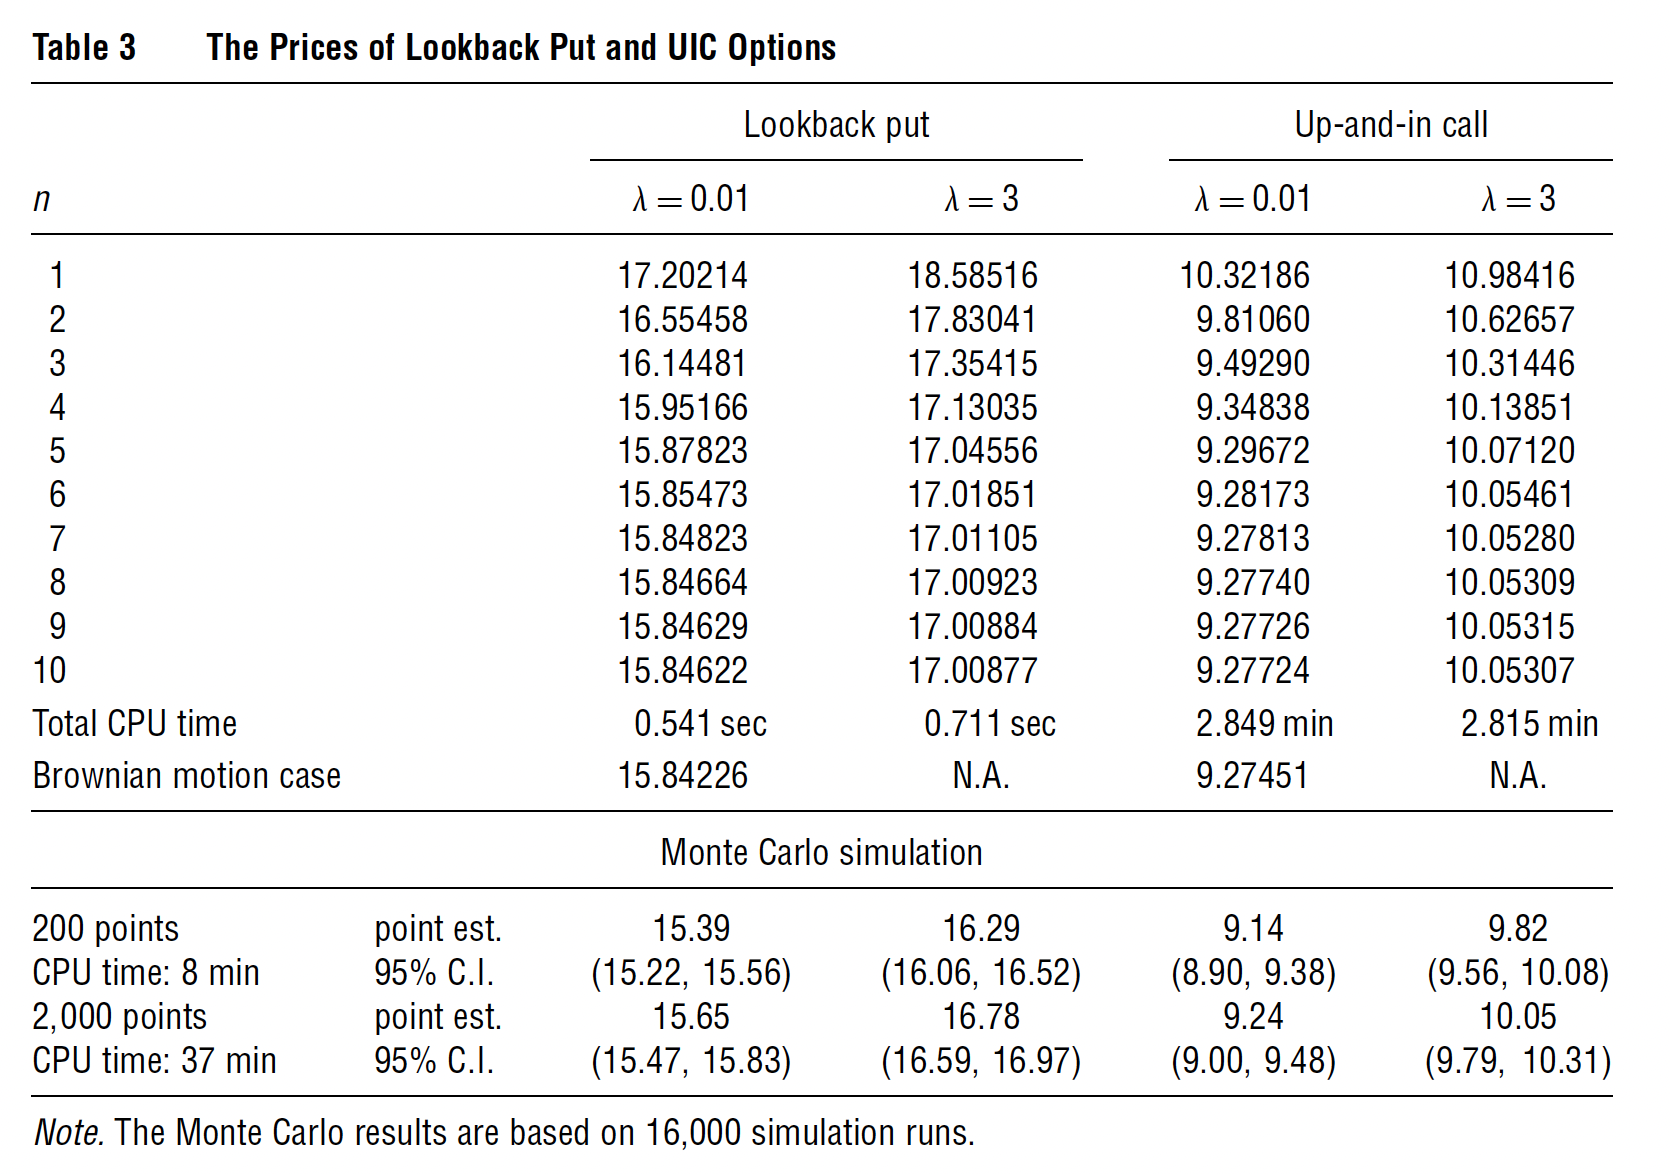
\includegraphics[width=0.7\textwidth]{1}
%     % \caption{This is a sample figure caption}
%     % \label{fig:example}
%     \end{figure}
    
% \end{frame}



\begin{frame}{Barrier Options}

    {\footnotesize \footnotesize
    \par Rewrite the pricing formula of up-and-in call option(UIC) in early silde:
    \begin{align*}
        UIC(k,T) = E^{\mathbb{P}^*} \left[ e^{-rT} \left( S(T) - e^{-k} \right)^+ I{[\tau_b < T]} \right]
    \end{align*}
    \par where \( H > S(0) \) is the barrier level, \( k = -\log(K) \) the transformed strike and \( b = \log(H/S(0)) \). In previous paper, we obtain:
    \begin{align*}
        UIC(k,T) = S(0) \tilde{\Psi}_{UI}(k,T) - Ke^{-rT} \Psi_{UI}(k,T)
    \end{align*}
    \par where:
    \begin{align*}
        \Psi_{UI}(k,T) = P^*(S(T) \geq e^{-k},  \tau_b < T), \quad \widetilde{\Psi}_{UI}(k,T) = \widetilde{P}(S(T) \geq e^{-k},  \tau_b < T) 
    \end{align*}
    \par Remark: Here we will relies on a two-dimensional Laplace transform for botth the option price and the probabilities. The formulae after doing two-dimensional 
    transforms become much simpler than the one-dimensional formulae in Kou and Wang (2003), which involve many special functions.
    }
    
\end{frame}


\begin{frame}{Barrier Options Con.}

    {\footnotesize \footnotesize
    \par Theorem:  For \(\xi\) and \(\alpha\) such that \(0 < \xi < \eta_1 - 1\) and \(\alpha > \max(G(\xi + 1) - r, 0)\) (such a choice of \(\xi\) and \(\alpha\) is possible 
    for all small enough \(\xi\) as \(G(1) - r = -\delta < 0\)). The Laplace transform with respect to \(k\) and \(T\) of \(UIC(k, T)\) is given by
    \begin{align*}
    \tilde{f}_{UIC}(\xi, \alpha) &= \int_{0}^{\infty} \int_{-\infty}^{\infty} e^{-\xi k - \alpha T} UIC(k, T) dk dT \\
    &= \frac{H^{\xi+1}}{\xi (\xi + 1)} \frac{1}{r + \alpha - G(\xi + 1)} \left( A(r + \alpha) \frac{\eta_1}{\eta_1 - (\xi + 1)} + B(r + \alpha) \right)
    \end{align*}
    \par where

    \begin{align*}
    A(h) &:= E^* \left[ e^{-h\tau_b} \mathbf{1}_{\{X(\tau_b) > b\}} \right] =
     \frac{(\eta_1 - \beta_{1,h}) (\beta_{2,h} - \eta_1)}{\eta_1 (\beta_{2,h} - \beta_{1,h})} \left[ e^{-b\beta_{1,h}} - e^{-b\beta_{2,h}} \right]\\
    B(h) &:= E^* \left[ e^{-h\tau_b} \mathbf{1}_{\{X(\tau_b = b)\}} \right] =
    \frac{\eta_1 - \beta_{1,h}}{\beta_{2,h} - \beta_{1,h}} e^{-b\beta_{1,h}} + \frac{\beta_{2,h} - \eta_1}{\beta_{2,h} - \beta_{1,h}} e^{-b\beta_{2,h}}
    \end{align*}
    \par with \(b = \log(H/S(0))\).
    }
    


\end{frame}


\begin{frame}{Barrier Options Con.}

    {\footnotesize \footnotesize
    \par  If \(0 < \xi < \eta_1\) and \(\alpha > \max(G(\xi), 0)\) (again this choice of \(\xi\) and \(\alpha\) is possible for 
    all \(\xi\) small enough as \(G(0) = 0\)), then the Laplace transform with respect to \(k\) and \(T\) of \(\Psi_{UI}(k, T)\) is:
     \vspace{1em}
    \begin{align*}
        \tilde{f}_{\Psi_{UI}}(\xi, \alpha) &= \int_0^{\infty} \left( \int_{-\infty}^{\infty} e^{-\xi k - \alpha T} \Psi_{UI}(k, T) dk \right) dT\\
    &= \frac{H^{\xi}}{\xi} \frac{1}{\alpha - G(\xi)} \left( A(\alpha) \frac{\eta_1}{\eta_1 - \xi} + B(\alpha) \right)
    \end{align*}

    \vspace{1em}
    \par The Laplace transforms with respect to \(k\) and \(T\) of \(\tilde{\Psi}_{UI}(k, T)\) is given 
    similarly with \(\tilde{G}\) replacing \(G\) and the functions \(\tilde{A}\) and \(\tilde{B}\) defined similarly. 
    To perform the inversion, They use the two-sided Euler method(EUL) as in Petrella (2004). Compare with GS method, EUL use standard double
     precision, get stable answers, and convergence is much faster.

    }
\end{frame}


\begin{frame}{Barrier Options Con.}

    {\footnotesize \footnotesize
    \par Statistical results:
    \vspace{1em}
    \par The author price up-and-in calls using the two-dimensional transform
     herein and compare the results with the one-dimensional transform in Kou and Wang (2003) (KW from now on and in the table) 
     and Monte Carlo simulation (MC). 
      \vspace{1em}
    \par For the two-dimensional transform, the price obtained in both inverting $ \tilde{f}_{UIC}(\xi, \alpha)$ and inverting $ \tilde{f}_{\Psi_{UI}}(\xi, \alpha)$.
     \vspace{1em}
    \par The two-dimensional Laplace transform approach is more efficient, simpler, and numerically 
    stable compared to Kou-Wang's GS inversion method, while achieving accuracy comparable to or better than Monte Carlo at a fraction of the computational cost.
    }   
\end{frame}

% \begin{frame}

%     {\footnotesize \footnotesize

%     }
    
% \end{frame}
% % {\mathbb{P}^*}
% \tilde{\mathbb{P}}
% {\footnotesize \footnotesize
% }
% \tiny
% \scriptsize
% \footnotesize
% \small
% \normalsize (default)
\end{document}